
\begin{table}[h!]
\centering
\scriptsize
\begin{tabular}{l|cc|cccc}
  \parbox[b][2mm]{33mm}{Model}  & 
  \parbox[b][2mm]{11mm}{\centering Residual}  &
  \parbox[b][4mm]{7mm }{\centering R\textsuperscript{2} }    &
  \parbox[b][4mm]{7mm }{\centering CVM 1se }  & 
  \parbox[b][4mm]{7mm }{\centering R\textsuperscript{2}  1se} & 
  \parbox[b][4mm]{7mm }{\centering CVM min }  & 
  \parbox[b][4mm]{7mm }{\centering R\textsuperscript{2}  min} 
        \\ \hline \hline
  Age, Manifold LDDMM  & 4.4  & 0.14 & -    & -    & -    & -    \\
  Age, Intensity VBM   & -    & -    & 4.9  & 0.24 & 4.8  & 0.95 \\
  Age, Transport VBM   & -    & -    & 4.5  & 0.39 & 4.3  & 0.72 \\ \hline
  MMSE, Manifold LDDMM & 3.8  & 0.15 & -    & -    & -    & -    \\
  MMSE, Intensity VBM  & -    & -    & 3.80 & 0.21 & 3.61 & 0.97 \\
  MMSE, Transport VBM  & -    & -    & 3.61 & 0.25 & 3.27 & 0.54 \\ \hline
  CDR, Manifold LDDMM  & 0.35 & 0.20 & -    & -    & -    & -    \\
  CDR, Intensity VBM   & -    & -    & 0.36 & 0.21 & 0.33 & 0.69 \\
  CDR, Transport VBM   & -    & -    & 0.32 & 0.40 & 0.30 & 0.72 \\
\end{tabular} 
\caption{ \label{fig:prediction}  Elastic net regression on transport cost
and mass allocation images versus intensity images and comparison to linear
models based on a global deformation approach. (p--value 0) and for MMSE 1.1 times (p-value 0.03) based on 1000
permutations.} 
\vspace{-10mm}
\end{table}



\begin{figure}[h!]
\centering
\scriptsize
\begin{tabular}{cc}
\begin{tabular}{l|cc|cccc}
  \parbox[b][2mm]{33mm}{Model}  & 
  \parbox[b][2mm]{11mm}{\centering Residual}  &
  \parbox[b][4mm]{7mm }{\centering R\textsuperscript{2} }    &
  \parbox[b][4mm]{7mm }{\centering CVM 1se }  & 
  \parbox[b][4mm]{7mm }{\centering R\textsuperscript{2}  1se} & 
  \parbox[b][4mm]{7mm }{\centering CVM min }  & 
  \parbox[b][4mm]{7mm }{\centering R\textsuperscript{2}  min} 
        \\ \hline \hline
\scriptsize
  Age, Manifold LDDMM  & 4.4  & 0.14 & -    & -    & -    & -    \\
  Age, Intensity VBM   & -    & -    & 4.9  & 0.24 & 4.8  & 0.95 \\
  Age, Transport VBM   & -    & -    & 4.5  & 0.39 & 4.3  & 0.72 \\ \hline
  MMSE, Manifold LDDMM & 3.8  & 0.15 & -    & -    & -    & -    \\
  MMSE, Intensity VBM  & -    & -    & 3.80 & 0.21 & 3.61 & 0.97 \\
  MMSE, Transport VBM  & -    & -    & 3.61 & 0.25 & 3.27 & 0.54 \\ \hline
  CDR, Manifold LDDMM  & 0.35 & 0.20 & -    & -    & -    & -    \\
  CDR, Intensity VBM   & -    & -    & 0.36 & 0.21 & 0.33 & 0.69 \\
  CDR, Transport VBM   & -    & -    & 0.32 & 0.40 & 0.30 & 0.72 \\
\end{tabular} 
&
  \raisebox{-13.5mm}{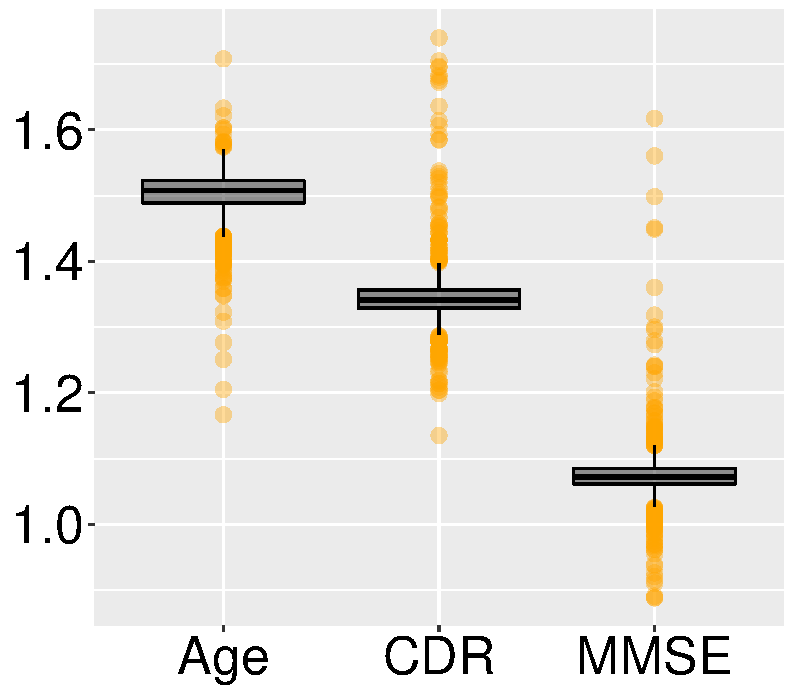
\includegraphics[width=34mm]{glmnet-cvm-permutations}}
\\
        \footnotesize{ (a) } & \footnotesize{ (b) }
\end{tabular}
\caption{ \label{fig:prediction} (b) Elastic net regression on transport cost
and mass allocation images versus intensity images and comparison to linear
models based on a global deformation approach.(a) Permutation test for the
transport based regression fits. The y-Axis show the distribution of the
permuted CVM scaled by the non-permuted CVM, thus for Age the permuted results
are on average 1.5 times above the non-permuted fit (p--value 0), for CDR 1.35
times (p--value 0) and for MMSE 1.1 times (p-value 0.03) based on 1000
permutations.} 
\vspace{-7mm}
\end{figure}


\begingroup
\newcolumntype{M}[1]{>{\centering\arraybackslash}m{#1}}
%\scriptsize
\renewcommand{\arraystretch}{0}
\setlength{\tabcolsep}{0pt}
\begin{figure}[h!]
\centering
\begin{tabular}{r}
\begin{tabular}{lcr}
        \multicolumn{3}{c}{\parbox[t][3mm]{20mm}{Pearson's r } }\\
        \parbox[t][3mm]{7mm}{-0.7} & 
        
\includegraphics[width=0.8\linewidth]{colorbar} & 
        \parbox[t][3mm]{6mm}{\hfill 0.7}
\end{tabular}\\
  \begin{tabular}{l||ccc||ccc||ccc} 
 \multirow{2}{*}{\rotatebox[origin=c]{90}{Age}}&
 %   \rotatebox[origin=c]{90}{G}&
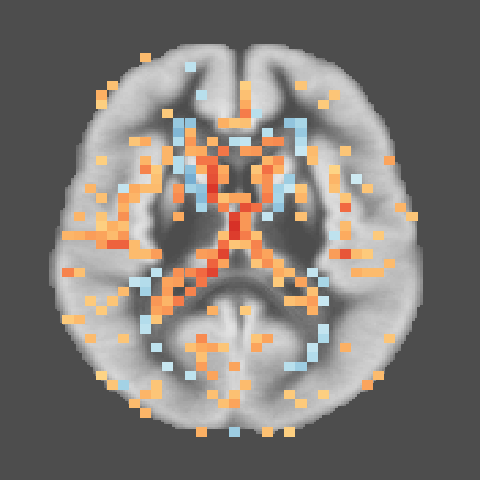
\includegraphics[width=0.1\linewidth]{cor-axial-age-t-iG} &
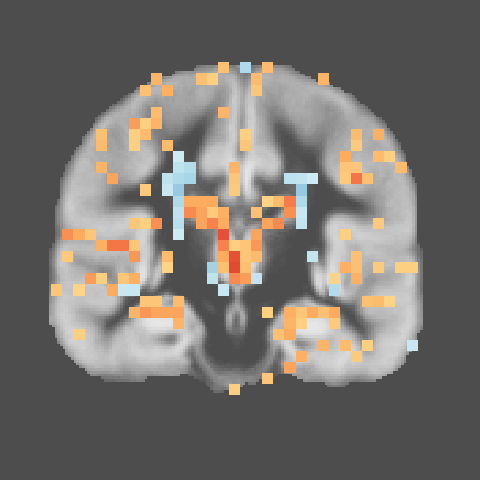
\includegraphics[width=0.1\linewidth]{cor-coronal-age-t-iG} &
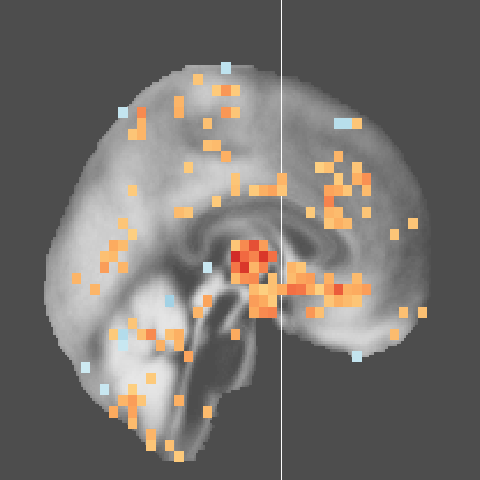
\includegraphics[width=0.1\linewidth]{cor-sagital-age-t-iG} &

\includegraphics[width=0.1\linewidth]{cor-axial-age-t-mG} &

\includegraphics[width=0.1\linewidth]{cor-coronal-age-t-mG} &
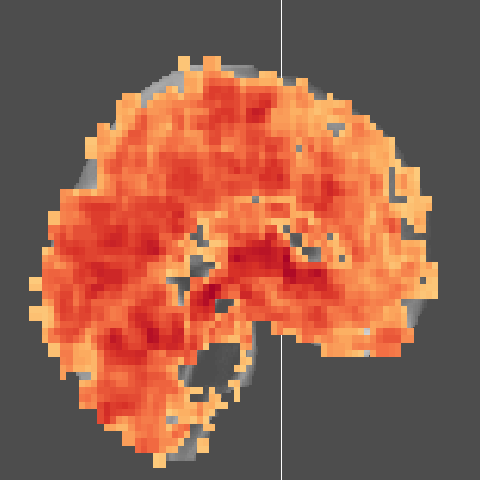
\includegraphics[width=0.1\linewidth]{cor-sagital-age-t-mG} &
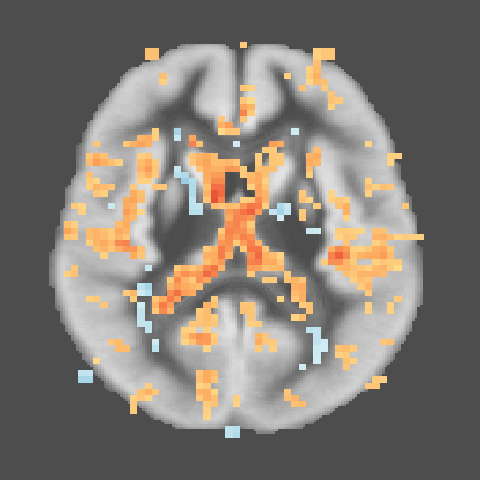
\includegraphics[width=0.1\linewidth]{cor-axial-age-t-tG} &
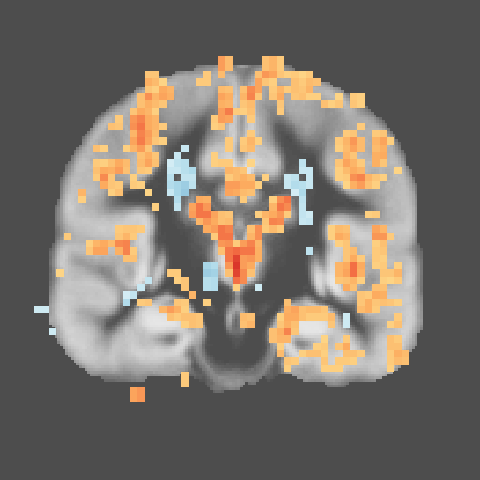
\includegraphics[width=0.1\linewidth]{cor-coronal-age-t-tG} &
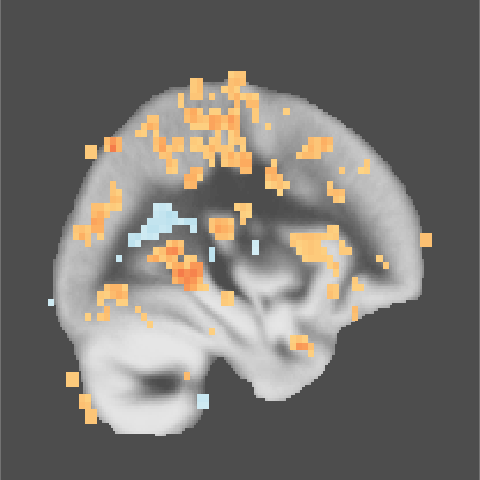
\includegraphics[width=0.1\linewidth]{cor-sagital-age-t-tG} 
  \\
  &
%    \rotatebox[origin=c]{90}{W}&
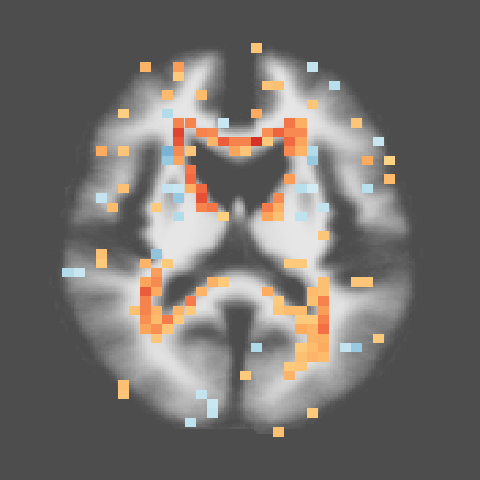
\includegraphics[width=0.1\linewidth]{cor-axial-age-t-iW} &
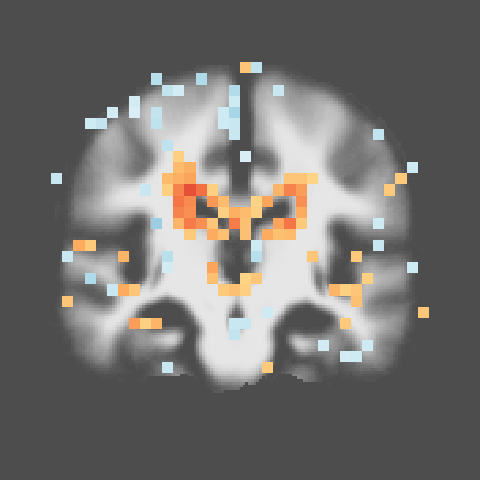
\includegraphics[width=0.1\linewidth]{cor-coronal-age-t-iW} &
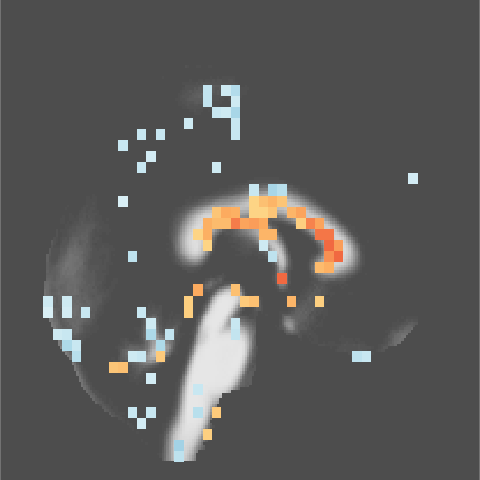
\includegraphics[width=0.1\linewidth]{cor-sagital-age-t-iW} &
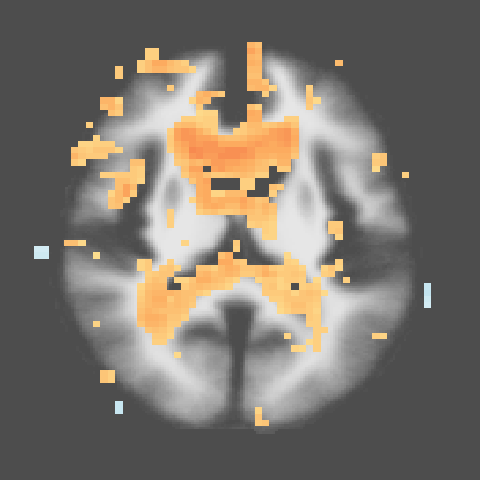
\includegraphics[width=0.1\linewidth]{cor-axial-age-t-mW} &
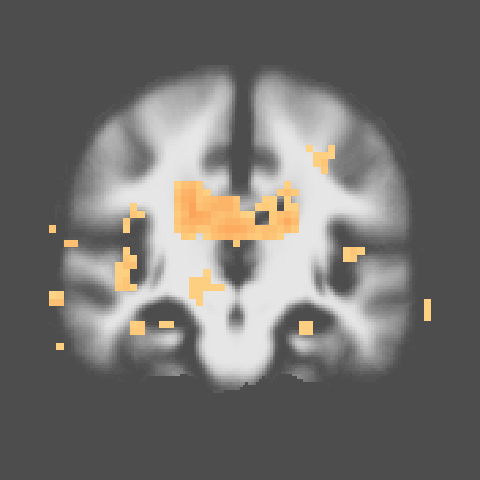
\includegraphics[width=0.1\linewidth]{cor-coronal-age-t-mW} &
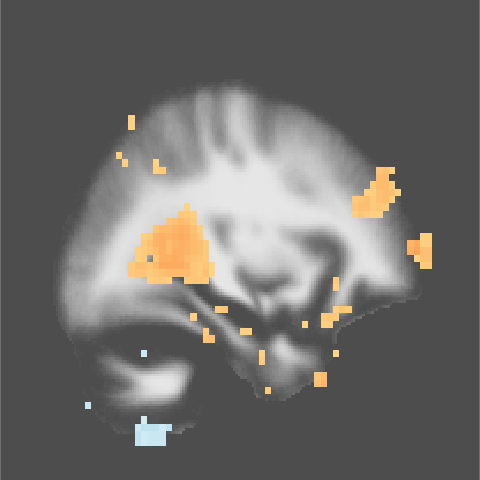
\includegraphics[width=0.1\linewidth]{cor-sagital-age-t-mW} &
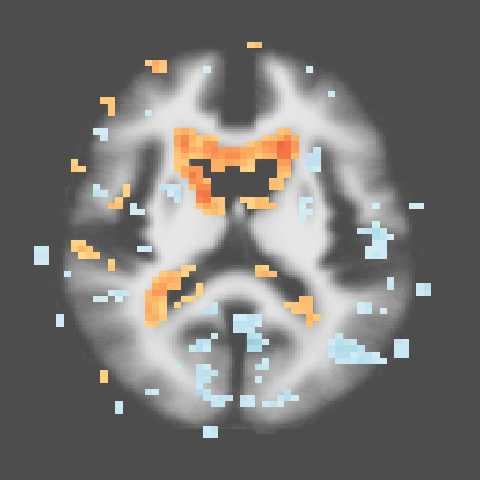
\includegraphics[width=0.1\linewidth]{cor-axial-age-t-tW} &
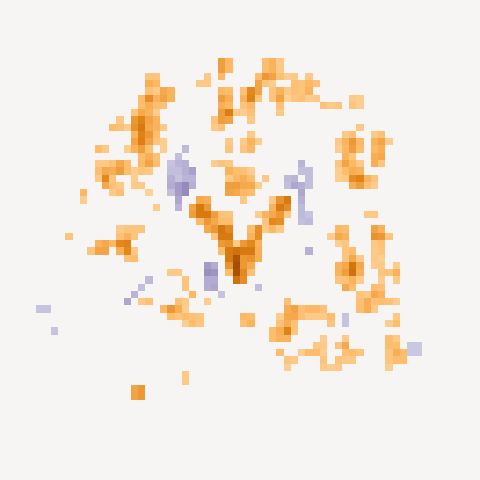
\includegraphics[width=0.1\linewidth]{cor-coronal-age-t-tW} &
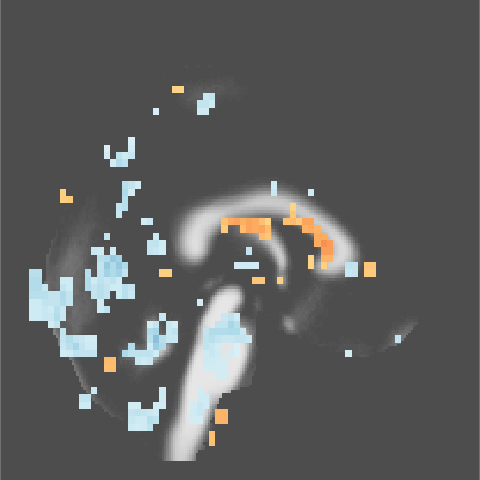
\includegraphics[width=0.1\linewidth]{cor-sagital-age-t-tW} 
  \\ \hline 
\multirow{2}{*}{\rotatebox[origin=c]{90}{CDR}}&
%    \rotatebox[origin=c]{90}{G}&
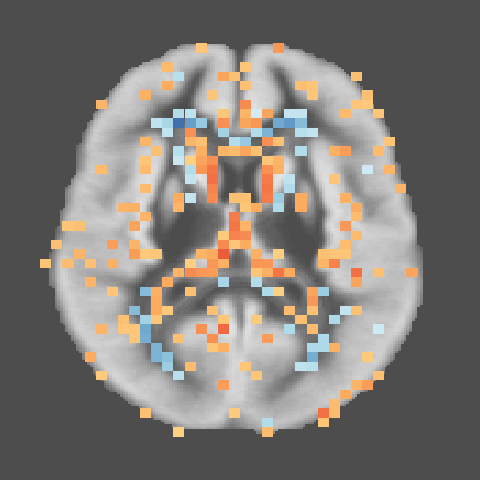
\includegraphics[width=0.1\linewidth]{cor-axial-cdr-t-iG} &
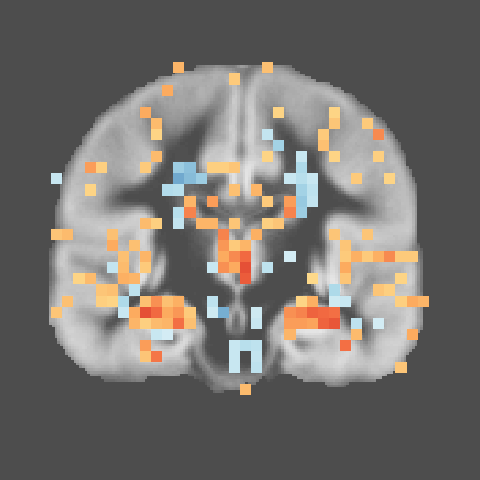
\includegraphics[width=0.1\linewidth]{cor-coronal-cdr-t-iG} &
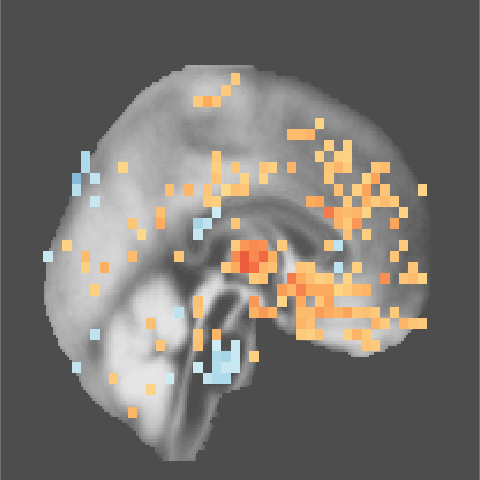
\includegraphics[width=0.1\linewidth]{cor-sagital-cdr-t-iG} &
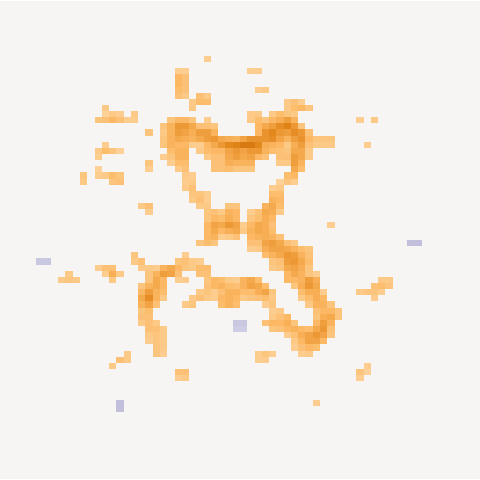
\includegraphics[width=0.1\linewidth]{cor-axial-cdr-t-mG} &

\includegraphics[width=0.1\linewidth]{cor-coronal-cdr-t-mG} &
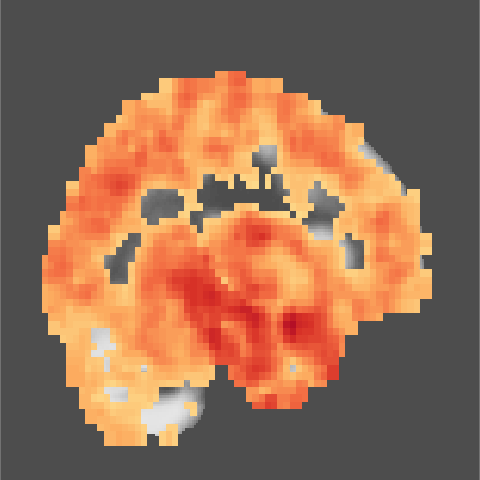
\includegraphics[width=0.1\linewidth]{cor-sagital-cdr-t-mG} &
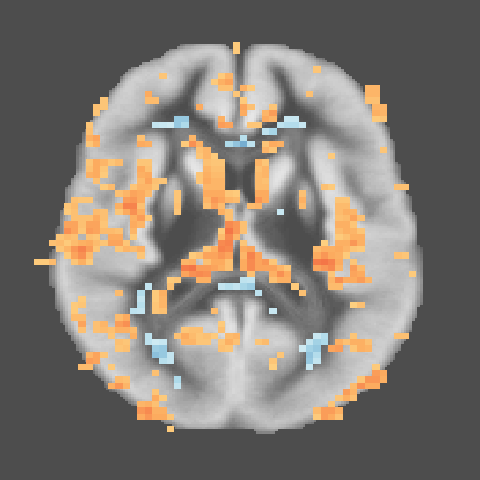
\includegraphics[width=0.1\linewidth]{cor-axial-cdr-t-tG} &
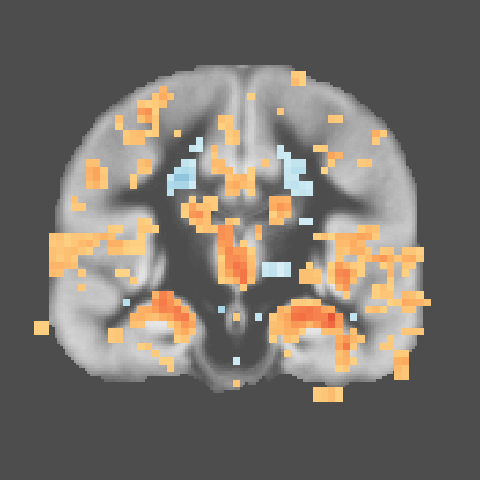
\includegraphics[width=0.1\linewidth]{cor-coronal-cdr-t-tG} &
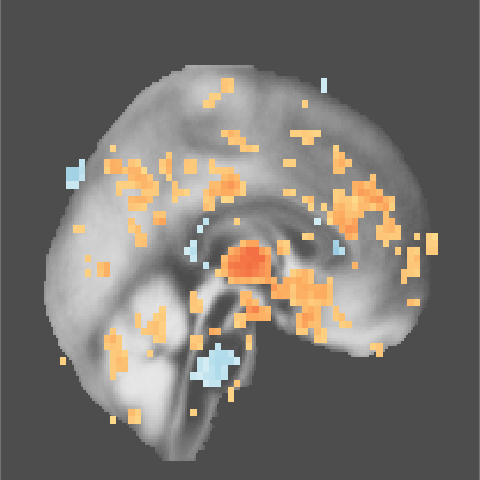
\includegraphics[width=0.1\linewidth]{cor-sagital-cdr-t-tG} 
  \\
  &
%    \rotatebox[origin=c]{90}{W}&
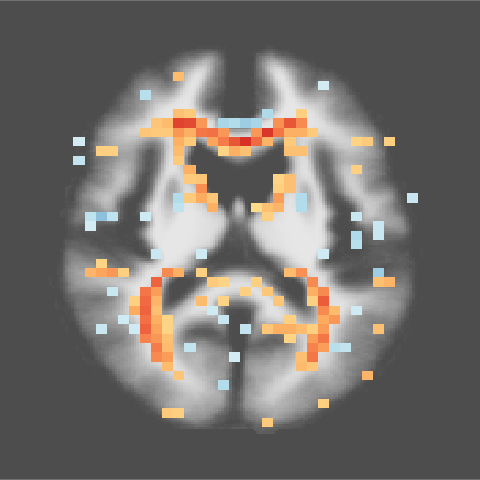
\includegraphics[width=0.1\linewidth]{cor-axial-cdr-t-iW} &
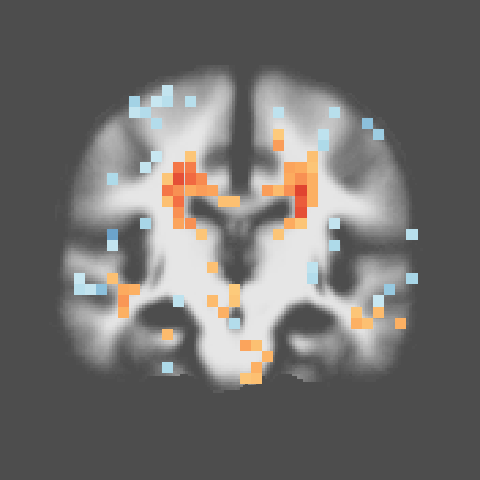
\includegraphics[width=0.1\linewidth]{cor-coronal-cdr-t-iW} &
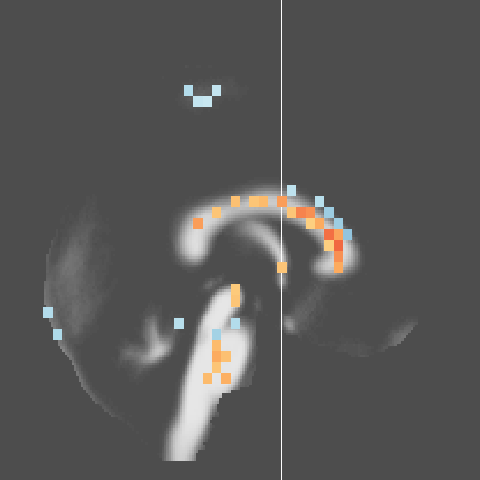
\includegraphics[width=0.1\linewidth]{cor-sagital-cdr-t-iW} &
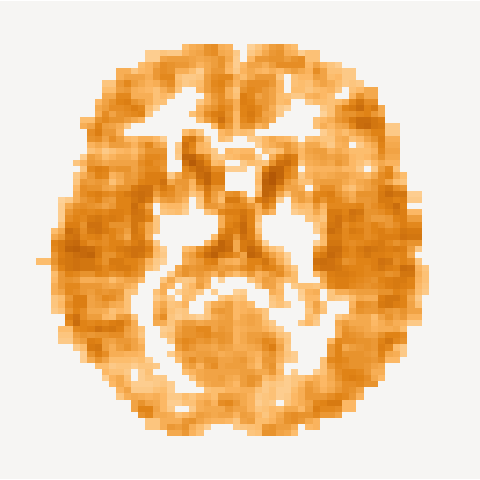
\includegraphics[width=0.1\linewidth]{cor-axial-cdr-t-mW} &
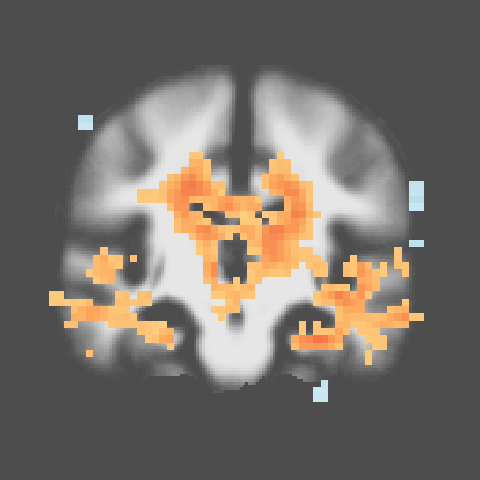
\includegraphics[width=0.1\linewidth]{cor-coronal-cdr-t-mW} &
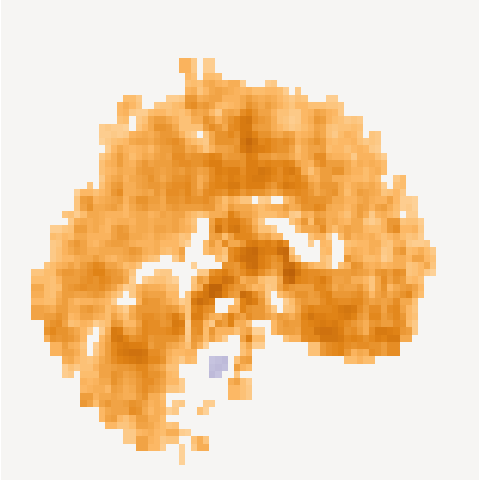
\includegraphics[width=0.1\linewidth]{cor-sagital-cdr-t-mW} &
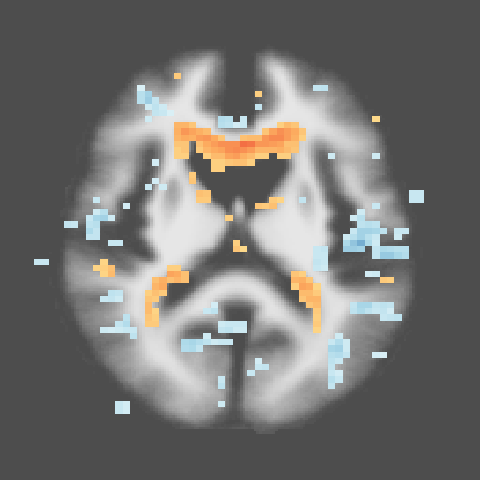
\includegraphics[width=0.1\linewidth]{cor-axial-cdr-t-tW} &
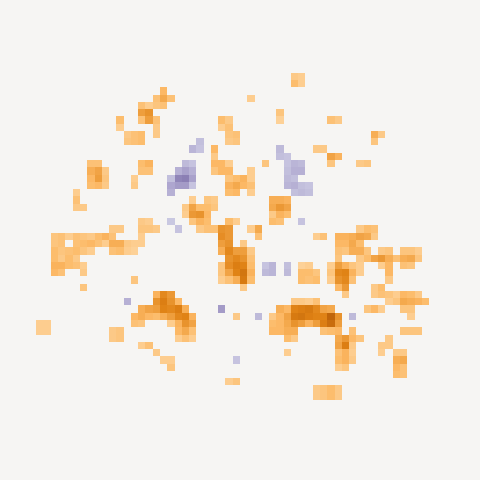
\includegraphics[width=0.1\linewidth]{cor-coronal-cdr-t-tW} &
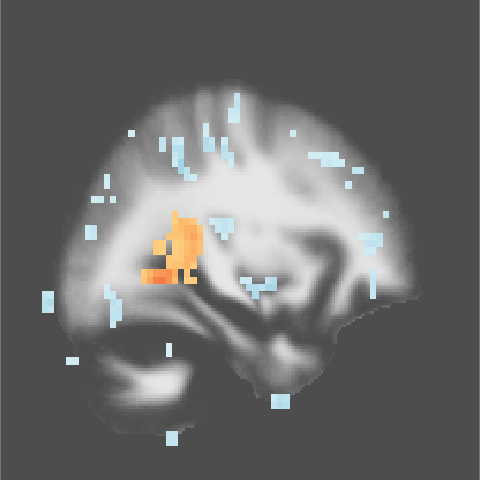
\includegraphics[width=0.1\linewidth]{cor-sagital-cdr-t-tW} 
  \\ \hline 
  \multirow{2}{*}{\rotatebox[origin=c]{90}{MMSE}} &
%    \rotatebox[origin=c]{90}{G}&
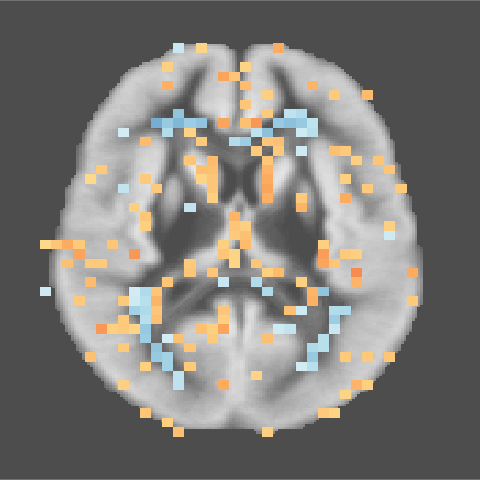
\includegraphics[width=0.1\linewidth]{cor-axial-mmse-t-iG} &
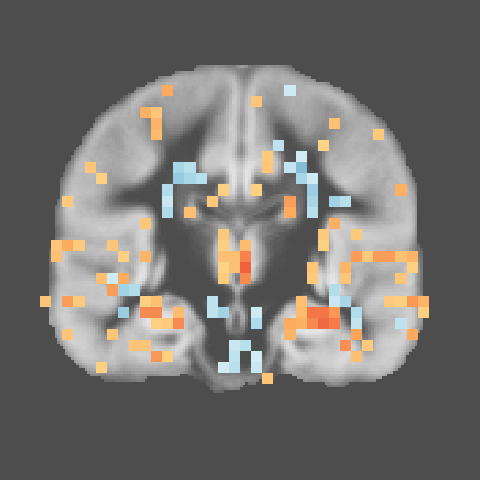
\includegraphics[width=0.1\linewidth]{cor-coronal-mmse-t-iG} &
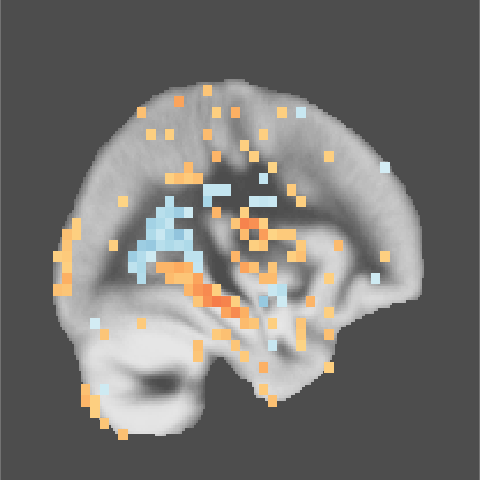
\includegraphics[width=0.1\linewidth]{cor-sagital-mmse-t-iG} &

\includegraphics[width=0.1\linewidth]{cor-axial-mmse-t-mG} &

\includegraphics[width=0.1\linewidth]{cor-coronal-mmse-t-mG} &
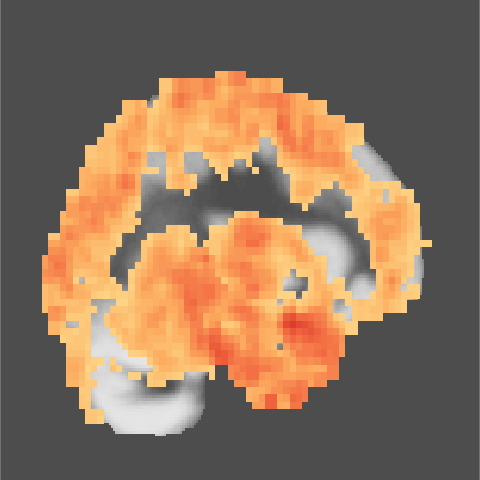
\includegraphics[width=0.1\linewidth]{cor-sagital-mmse-t-mG} &
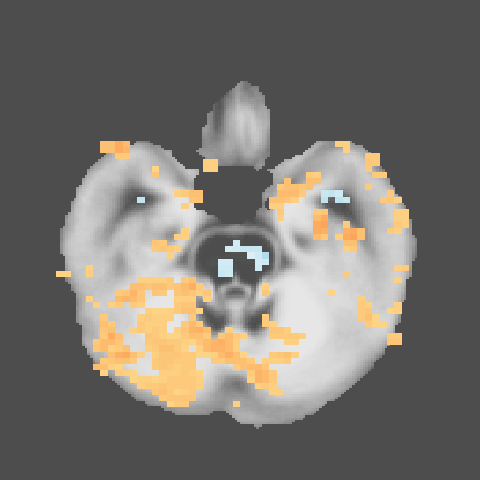
\includegraphics[width=0.1\linewidth]{cor-axial-mmse-t-tG} &
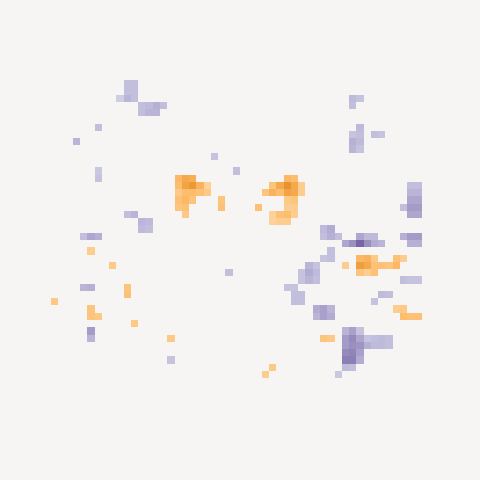
\includegraphics[width=0.1\linewidth]{cor-coronal-mmse-t-tG} &
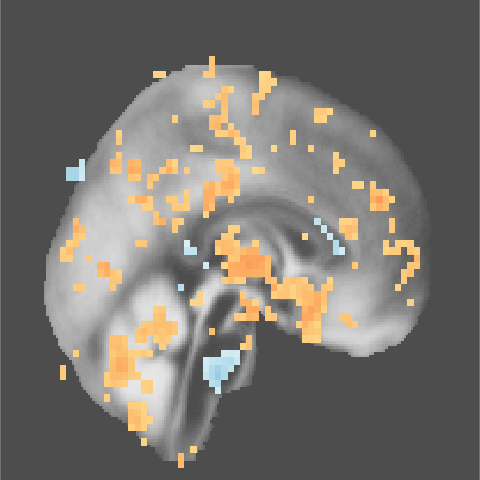
\includegraphics[width=0.1\linewidth]{cor-sagital-mmse-t-tG} 
  \\ 
  &
%    \rotatebox[origin=c]{90}{W}&
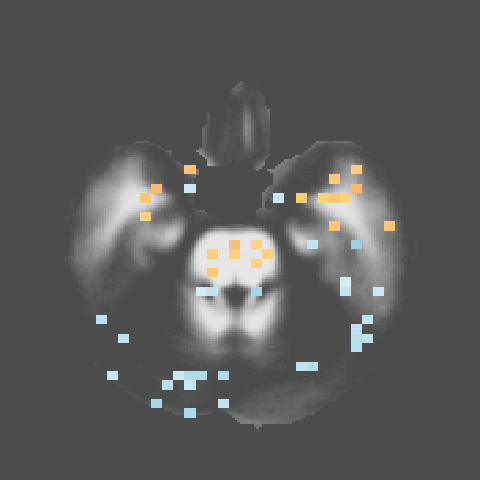
\includegraphics[width=0.1\linewidth]{cor-axial-mmse-t-iW} &
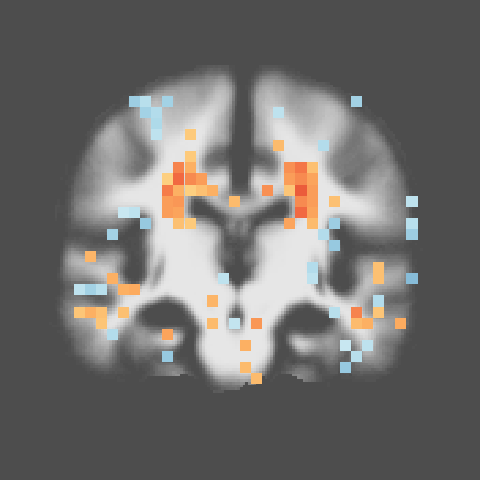
\includegraphics[width=0.1\linewidth]{cor-coronal-mmse-t-iW} &
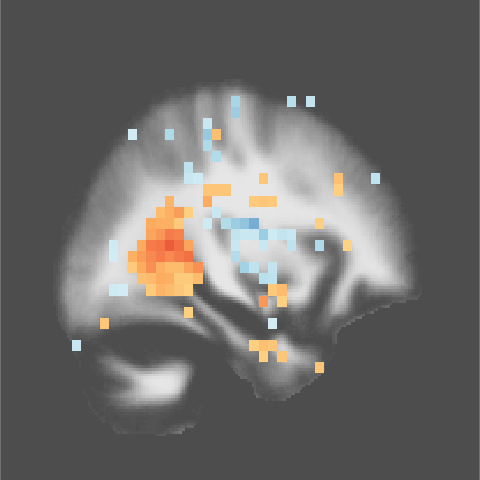
\includegraphics[width=0.1\linewidth]{cor-sagital-mmse-t-iW} &
\includegraphics[width=0.1\linewidth]{cor-axial-mmse-t-mW} &
\includegraphics[width=0.1\linewidth]{cor-coronal-mmse-t-mW} &
\includegraphics[width=0.1\linewidth]{cor-sagital-mmse-t-mW} &
\includegraphics[width=0.1\linewidth]{cor-axial-mmse-t-tW} &
\includegraphics[width=0.1\linewidth]{cor-coronal-mmse-t-tW} &
\includegraphics[width=0.1\linewidth]{cor-sagital-mmse-t-tW} 
  \\ \hline  \hline
  & \multicolumn{3}{c||}{Voxel Intensity}
  & \multicolumn{3}{c||}{Mass Imbalance}
  & \multicolumn{3}{c}{Transport Cost}
\end{tabular}
\end{tabular}
\caption{\label{fig:cor-oasis}
Correlation of Age, MMSE and CDR with smoothed segmentation mask intensity,
optimal transport mass imbalances and optimal transport costs of gray and white
matter.  Correlations are only shown at locations permutation tested p--value
less than 0.05. The background image are average white and gray matter
segmentations. 
\vspace{-7mm}
} 
\end{figure} 
\endgroup


\begingroup
\renewcommand{\arraystretch}{0}
\setlength{\tabcolsep}{0pt}
\begin{figure}[h!]
\centering
\begin{tabular}{r}
\begin{tabular}{lcr}
        \multicolumn{3}{c}{\parbox[t][3mm]{20mm}{Pearson's r } }\\
        \parbox[t][3mm]{7mm}{-0.7} & 
        \includegraphics[width=0.7\linewidth]{colorbar} & 
        \parbox[t][3mm]{6mm}{\hfill 0.7}
\end{tabular}\\
\begin{tabular}{l|cc|cc|cc} 
\parbox[t]{4mm}{\multirow{3}{*}{\rotatebox[origin=c]{90}{Voxel Intensity}}}&
\includegraphics[width=0.13\linewidth]{cor-axial-age-t-iG} &
\includegraphics[width=0.13\linewidth]{cor-axial-age-t-iW} &
\includegraphics[width=0.13\linewidth]{cor-axial-cdr-t-iG} &
\includegraphics[width=0.13\linewidth]{cor-axial-cdr-t-iW} &
\includegraphics[width=0.13\linewidth]{cor-axial-mmse-t-iG} &
\includegraphics[width=0.13\linewidth]{cor-axial-mmse-t-iW} \\ 
%
        &
\includegraphics[width=0.13\linewidth]{cor-coronal-age-t-iG} &
\includegraphics[width=0.13\linewidth]{cor-coronal-age-t-iW} &
\includegraphics[width=0.13\linewidth]{cor-coronal-cdr-t-iG} &
\includegraphics[width=0.13\linewidth]{cor-coronal-cdr-t-iW} &
\includegraphics[width=0.13\linewidth]{cor-coronal-mmse-t-iG} &
\includegraphics[width=0.13\linewidth]{cor-coronal-mmse-t-iW} \\ 
%
        &
\includegraphics[width=0.13\linewidth]{cor-sagital-age-t-iG} &
\includegraphics[width=0.13\linewidth]{cor-sagital-age-t-iW} &
\includegraphics[width=0.13\linewidth]{cor-sagital-cdr-t-iG} &
\includegraphics[width=0.13\linewidth]{cor-sagital-cdr-t-iW} &
\includegraphics[width=0.13\linewidth]{cor-sagital-mmse-t-iG} &
\includegraphics[width=0.13\linewidth]{cor-sagital-mmse-t-iW} \\ \hline \hline
%%
\parbox[t]{4mm}{\multirow{3}{*}{\rotatebox[origin=c]{90}{Mass Imbalance}}}&
\includegraphics[width=0.13\linewidth]{cor-axial-age-t-mG} &
\includegraphics[width=0.13\linewidth]{cor-axial-age-t-mW} &
\includegraphics[width=0.13\linewidth]{cor-axial-cdr-t-mG} &
\includegraphics[width=0.13\linewidth]{cor-axial-cdr-t-mW} &
\includegraphics[width=0.13\linewidth]{cor-axial-mmse-t-mG} &
\includegraphics[width=0.13\linewidth]{cor-axial-mmse-t-mW} \\ 
%
        &
\includegraphics[width=0.13\linewidth]{cor-coronal-age-t-mG} &
\includegraphics[width=0.13\linewidth]{cor-coronal-age-t-mW} &
\includegraphics[width=0.13\linewidth]{cor-coronal-cdr-t-mG} &
\includegraphics[width=0.13\linewidth]{cor-coronal-cdr-t-mW} &
\includegraphics[width=0.13\linewidth]{cor-coronal-mmse-t-mG} &
\includegraphics[width=0.13\linewidth]{cor-coronal-mmse-t-mW} \\ 
%
        &
\includegraphics[width=0.13\linewidth]{cor-sagital-age-t-mG} &
\includegraphics[width=0.13\linewidth]{cor-sagital-age-t-mW} &
\includegraphics[width=0.13\linewidth]{cor-sagital-cdr-t-mG} &
\includegraphics[width=0.13\linewidth]{cor-sagital-cdr-t-mW} &
\includegraphics[width=0.13\linewidth]{cor-sagital-mmse-t-mG} &
\includegraphics[width=0.13\linewidth]{cor-sagital-mmse-t-mW} \\ \hline \hline
%%
\parbox[t]{2mm}{\multirow{3}{*}{\rotatebox[origin=c]{90}{Transport Cost}}}&
\includegraphics[width=0.13\linewidth]{cor-axial-age-t-tG} &
\includegraphics[width=0.13\linewidth]{cor-axial-age-t-tW} &
\includegraphics[width=0.13\linewidth]{cor-axial-cdr-t-tG} &
\includegraphics[width=0.13\linewidth]{cor-axial-cdr-t-tW} &
\includegraphics[width=0.13\linewidth]{cor-axial-mmse-t-tG} &
\includegraphics[width=0.13\linewidth]{cor-axial-mmse-t-tW} \\ 
%
        &
\includegraphics[width=0.13\linewidth]{cor-coronal-age-t-tG} &
\includegraphics[width=0.13\linewidth]{cor-coronal-age-t-tW} &
\includegraphics[width=0.13\linewidth]{cor-coronal-cdr-t-tG} &
\includegraphics[width=0.13\linewidth]{cor-coronal-cdr-t-tW} &
\includegraphics[width=0.13\linewidth]{cor-coronal-mmse-t-tG} &
\includegraphics[width=0.13\linewidth]{cor-coronal-mmse-t-tW} \\ 
%
        &
\includegraphics[width=0.13\linewidth]{cor-sagital-age-t-tG} &
\includegraphics[width=0.13\linewidth]{cor-sagital-age-t-tW} &
\includegraphics[width=0.13\linewidth]{cor-sagital-cdr-t-tG} &
\includegraphics[width=0.13\linewidth]{cor-sagital-cdr-t-tW} &
\includegraphics[width=0.13\linewidth]{cor-sagital-mmse-t-tG} &
\includegraphics[width=0.13\linewidth]{cor-sagital-mmse-t-tW} \\ \hline \hline
%
& \parbox[b][4mm]{12mm}{Age(w)} 
& \parbox[b][4mm]{12mm}{Age(g)} 
& \parbox[b][4mm]{15mm}{CDR(w)} 
& \parbox[b][4mm]{15mm}{CDR(g) }
& \parbox[b][4mm]{15mm}{-MMSE(w)}
& \parbox[b][4mm]{15mm}{-MMSE(g)}
\end{tabular}
\end{tabular}
\caption{\label{fig:cor-oasis}
Correlation of Age, MMSE and CDR with smoothed segmentation mask intensity,
optimal transport mass imbalances and optimal transport costs of gray and white
matter.  Correlations are only shown at locations permutation tested p--value
less than 0.05. The background image are average white and gray matter
segmentations. 
} 
\end{figure} \endgroup





\begin{figure}[htb]
\scriptsize
\begin{tabular}{cc}
\raisebox{-15mm}{\includegraphics[width=34mm]{glmnet-cvm-permutations}}
        &
\begin{tabular}{l|cccc|cc}
\parbox[2mm]{33mm}{Model}  & 
\parbox[2mm]{11mm}{\centering Residual} & 
\parbox[2mm]{5mm }{\centering $R^2$} & 
\parbox[2mm]{5mm }{\centering F}   & 
\parbox[2mm]{11mm}{\centering p--value}   & 
\parbox[2mm]{7mm }{\centering CVM }  & 
\parbox[2mm]{7mm }{\centering $l_1 R^2$} 
        \\ \hline \hline
\scriptsize
  Age, Manifold LDDMM  & 4.4  & 0.14  & 9.9  & 1.0e-4      & NA    & NA   \\
  Age, Intensity VBM   & 2.4  & 0.86  & 17.4 & $<\epsilon$ & 4.9   & 0.24 \\
  Age, Transport VBM   & 3.1  & 0.74  & 11.1 & $<\epsilon$ & 4.5   & 0.39 \\ \hline
  MMSE, Manifold LDDMM & 3.8  & 0.15  & 20.9 & 1.2e-5      & NA    & NA   \\
  MMSE, Intensity VBM  & 3.0  & 0.50  &  5.6 & 2.1e-10     & 3.80  & 0.21 \\
  MMSE, Transport VBM  & 3.0  & 0.50  & 11.2 & 3.3e-13     & 3.61  & 0.25 \\ \hline
  CDR, Manifold LDDMM  & 0.35 & 0.20  & 30.0 & 2.4e-7      & NA    & NA   \\
  CDR, Intensity VBM   & 0.19 & 0.79  & 19.5 & $<\epsilon$ & 0.36  & 0.21 \\
  CDR, Transport VBM   & 0.26 & 0.61  & 8.5  & 5.2e-15     & 0.32  & 0.40 \\
\end{tabular} \\
        \footnotesize{ (a) } & \footnotesize{ (b) }
\end{tabular}
\caption{ \label{fig:prediction} Prediction with elastic net and comparison to
linear models based on the LDDMM manifold approach.} 
\end{figure}

mmse permuted p-value 0.03, other 0

\secti





\begingroup
\renewcommand{\arraystretch}{0}
\setlength{\tabcolsep}{0pt}
\begin{figure}[bth]
\centering
\begin{tabular}{l|cc|cc|cc} 
\parbox[t]{4mm}{\multirow{3}{*}{\rotatebox[origin=c]{90}{Mass Imbalance}}}&
\includegraphics[width=0.16\linewidth]{cor-axial-age-mW} &
\includegraphics[width=0.16\linewidth]{cor-axial-age-t-mW} &
\includegraphics[width=0.16\linewidth]{cor-axial-cdr-mW} &
\includegraphics[width=0.16\linewidth]{cor-axial-cdr-t-mW} &
\includegraphics[width=0.16\linewidth]{cor-axial-mmse-mW} &
\includegraphics[width=0.16\linewidth]{cor-axial-mmse-t-mW} \\ 
%
        &
\includegraphics[width=0.16\linewidth]{cor-coronal-age-mW} &
\includegraphics[width=0.16\linewidth]{cor-coronal-age-t-mW} &
\includegraphics[width=0.16\linewidth]{cor-coronal-cdr-mW} &
\includegraphics[width=0.16\linewidth]{cor-coronal-cdr-t-mW} &
\includegraphics[width=0.16\linewidth]{cor-coronal-mmse-mW} &
\includegraphics[width=0.16\linewidth]{cor-coronal-mmse-t-mW} \\ 
%
        &
\includegraphics[width=0.16\linewidth]{cor-sagital-age-mW} &
\includegraphics[width=0.16\linewidth]{cor-sagital-age-t-mW} &
\includegraphics[width=0.16\linewidth]{cor-sagital-cdr-mW} &
\includegraphics[width=0.16\linewidth]{cor-sagital-cdr-t-mW} &
\includegraphics[width=0.16\linewidth]{cor-sagital-mmse-mW} &
\includegraphics[width=0.16\linewidth]{cor-sagital-mmse-t-mW} \\ \hline \hline
%
\parbox[t]{2mm}{\multirow{3}{*}{\rotatebox[origin=c]{90}{Transport Cost}}}&
\includegraphics[width=0.16\linewidth]{cor-axial-age-tW} &
\includegraphics[width=0.16\linewidth]{cor-axial-age-t-tW} &
\includegraphics[width=0.16\linewidth]{cor-axial-cdr-tW} &
\includegraphics[width=0.16\linewidth]{cor-axial-cdr-t-tW} &
\includegraphics[width=0.16\linewidth]{cor-axial-mmse-tW} &
\includegraphics[width=0.16\linewidth]{cor-axial-mmse-t-tW} \\ 
%
        &
\includegraphics[width=0.16\linewidth]{cor-coronal-age-tW} &
\includegraphics[width=0.16\linewidth]{cor-coronal-age-t-tW} &
\includegraphics[width=0.16\linewidth]{cor-coronal-cdr-tW} &
\includegraphics[width=0.16\linewidth]{cor-coronal-cdr-t-tW} &
\includegraphics[width=0.16\linewidth]{cor-coronal-mmse-tW} &
\includegraphics[width=0.16\linewidth]{cor-coronal-mmse-t-tW} \\ 
%
        &
\includegraphics[width=0.16\linewidth]{cor-sagital-age-tW} &
\includegraphics[width=0.16\linewidth]{cor-sagital-age-t-tW} &
\includegraphics[width=0.16\linewidth]{cor-sagital-cdr-tW} &
\includegraphics[width=0.16\linewidth]{cor-sagital-cdr-t-tW} &
\includegraphics[width=0.16\linewidth]{cor-sagital-mmse-tW} &
\includegraphics[width=0.16\linewidth]{cor-sagital-mmse-t-tW} \\ \hline \hline
%
& \parbox[b][4mm]{6mm}{Age} 
& \parbox[b][4mm]{6mm}{Age\textsuperscript{*}} 
& \parbox[b][4mm]{6mm}{CDR} 
& \parbox[b][4mm]{6mm}{CDR\textsuperscript{*}}
& \parbox[b][4mm]{6mm}{MMSE}
& \parbox[b][4mm]{6mm}{MMSE\textsuperscript{*}}
\end{tabular}
\caption{\label{fig:cor-oasis-gray}
Correlation of age, MMSE and CDR with optimal transport mass imbalances and
optimal transport costs of gray matter. The columns with a \textsuperscript{*}
only show the voxels were the correlation has a permutation tested p-value less
than 0.05  }
\end{figure}
\endgroup

\begingroup
\renewcommand{\arraystretch}{0}
\setlength{\tabcolsep}{0pt}
\begin{figure}[bth]
\centering
\begin{tabular}{l|cc|cc|cc}
\parbox[t]{4mm}{\multirow{3}{*}{\rotatebox[origin=c]{90}{Mass Imbalance}}}&
\includegraphics[width=0.16\linewidth]{cor-axial-age-mG} &
\includegraphics[width=0.16\linewidth]{cor-axial-age-t-mG} &
\includegraphics[width=0.16\linewidth]{cor-axial-cdr-mG} &
\includegraphics[width=0.16\linewidth]{cor-axial-cdr-t-mG} &
\includegraphics[width=0.16\linewidth]{cor-axial-mmse-mG} &
\includegraphics[width=0.16\linewidth]{cor-axial-mmse-t-mG} \\ 
%
        &
\includegraphics[width=0.16\linewidth]{cor-coronal-age-mG} &
\includegraphics[width=0.16\linewidth]{cor-coronal-age-t-mG} &
\includegraphics[width=0.16\linewidth]{cor-coronal-cdr-mG} &
\includegraphics[width=0.16\linewidth]{cor-coronal-cdr-t-mG} &
\includegraphics[width=0.16\linewidth]{cor-coronal-mmse-mG} &
\includegraphics[width=0.16\linewidth]{cor-coronal-mmse-t-mG} \\ 
%
        &
\includegraphics[width=0.16\linewidth]{cor-sagital-age-mG} &
\includegraphics[width=0.16\linewidth]{cor-sagital-age-t-mG} &
\includegraphics[width=0.16\linewidth]{cor-sagital-cdr-mG} &
\includegraphics[width=0.16\linewidth]{cor-sagital-cdr-t-mG} &
\includegraphics[width=0.16\linewidth]{cor-sagital-mmse-mG} &
\includegraphics[width=0.16\linewidth]{cor-sagital-mmse-t-mG} \\ \hline \hline
%
\parbox[t]{2mm}{\multirow{3}{*}{\rotatebox[origin=c]{90}{Transport Cost}}}&
\includegraphics[width=0.16\linewidth]{cor-axial-age-tG} &
\includegraphics[width=0.16\linewidth]{cor-axial-age-t-tG} &
\includegraphics[width=0.16\linewidth]{cor-axial-cdr-tG} &
\includegraphics[width=0.16\linewidth]{cor-axial-cdr-t-tG} &
\includegraphics[width=0.16\linewidth]{cor-axial-mmse-tG} &
\includegraphics[width=0.16\linewidth]{cor-axial-mmse-t-tG} \\ 
%
        &
\includegraphics[width=0.16\linewidth]{cor-coronal-age-tG} &
\includegraphics[width=0.16\linewidth]{cor-coronal-age-t-tG} &
\includegraphics[width=0.16\linewidth]{cor-coronal-cdr-tG} &
\includegraphics[width=0.16\linewidth]{cor-coronal-cdr-t-tG} &
\includegraphics[width=0.16\linewidth]{cor-coronal-mmse-tG} &
\includegraphics[width=0.16\linewidth]{cor-coronal-mmse-t-tG} \\ 
%
        &
\includegraphics[width=0.16\linewidth]{cor-sagital-age-tG} &
\includegraphics[width=0.16\linewidth]{cor-sagital-age-t-tG} &
\includegraphics[width=0.16\linewidth]{cor-sagital-cdr-tG} &
\includegraphics[width=0.16\linewidth]{cor-sagital-cdr-t-tG} &
\includegraphics[width=0.16\linewidth]{cor-sagital-mmse-tG} &
\includegraphics[width=0.16\linewidth]{cor-sagital-mmse-t-tG} \\ \hline \hline
%%
& \parbox[b][4mm]{6mm}{Age} 
& \parbox[b][4mm]{6mm}{Age\textsuperscript{*}} 
& \parbox[b][4mm]{6mm}{CDR} 
& \parbox[b][4mm]{6mm}{CDR\textsuperscript{*}}
& \parbox[b][4mm]{6mm}{MMSE}
& \parbox[b][4mm]{6mm}{MMSE\textsuperscript{*}}
\end{tabular}
\caption{\label{fig:cor-oasis-white}
Correlation of age, MMSE and CDR with optimal transport mass imbalances and
optimal transport costs of white matter. The columns with a \textsuperscript{*}
only show the voxels were the correlation has a permutation tested p-value less
than 0.05  }
\end{figure}
\endgroup


%%%VBM glmnet /linear models
> ind <- get.selected.index(m.cdr$model)
> print( sqrt( m.cdr$model$cvm[ind$lambda.min] ) )
[1] 0.3369944
> print( m.cdr$model$glmnet.fit$dev.ratio[ind$lambda.min] )
[1] 0.5276706
> build.linear.model( cdr[cdr.index], all[cdr.index,ind$non.zero])$anova
Analysis of Variance Table

Response: y
           Df Sum Sq Mean Sq F value    Pr(>F)    
X1          1 1.8308 1.83076 48.8029 2.017e-10 ***
X2          1 2.6704 2.67043 71.1860 1.159e-13 ***
X3          1 1.1870 1.18697 31.6413 1.342e-07 ***
X4          1 1.7614 1.76136 46.9528 3.919e-10 ***
X5          1 1.8326 1.83258 48.8512 1.982e-10 ***
X6          1 1.3744 1.37444 36.6386 1.861e-08 ***
X7          1 1.1817 1.18169 31.5004 1.421e-07 ***
X8          1 0.6623 0.66228 17.6545 5.285e-05 ***
X9          1 0.1397 0.13965  3.7227 0.0561616 .  
X10         1 0.1610 0.16103  4.2926 0.0405350 *  
X11         1 0.8895 0.88950 23.7115 3.634e-06 ***
X12         1 0.5419 0.54187 14.4447 0.0002334 ***
X13         1 0.3259 0.32586  8.6866 0.0038885 ** 
X14         1 0.0633 0.06331  1.6876 0.1965444    
X15         1 0.4172 0.41721 11.1216 0.0011519 ** 
X16         1 0.1530 0.15301  4.0789 0.0457677 *  
X17         1 0.3900 0.38999 10.3961 0.0016476 ** 
X18         1 0.1350 0.13503  3.5995 0.0603283 .  
X19         1 0.2067 0.20674  5.5110 0.0206212 *  
X21         1 0.0823 0.08235  2.1951 0.1412046    
X22     ;
     double eyeClosingRadiusFactor =  1/7.0;
    1 0.0191 0.01907  0.5085 0.4772630    
X23         1 0.0743 0.07425  1.9794 0.1621720    
Residuals 114 4.2765 0.03751                      
---
Signif. codes:  0 ‘***’ 0.001 ‘**’ 0.01 ‘*’ 0.05 ‘.’ 0.1 ‘ ’ 1
> summary(  build.linear.model( cdr[cdr.index], all[cdr.index,ind$non.zero])$lm )

Call:
lm(formula = y ~ ., data = data.frame(y = y, x))

Residuals:
     Min       1Q   Median       3Q      Max 
-0.53460 -0.11300  0.00687  0.11912  0.39452 

Coefficients: (1 not defined because of singularities)
            Estimate Std. Error t value Pr(>|t|)    
(Intercept)  1.35161    0.10524  12.843  < 2e-16 ***
X1          -0.22982    0.08038  -2.859 0.005051 ** 
X2          -0.13452    0.06163  -2.183 0.031113 *  
X3          -0.07904    0.09291  -0.851 0.396691    
X4          -0.09599    0.06301  -1.523 0.130434    
X5          -0.03280    0.06564  -0.500 0.618281    
X6           1.02841    0.22170   4.639 9.42e-06 ***
X7          -0.01586    0.05894  -0.269 0.788312    
X8          -0.04065    0.06851  -0.593 0.554060    
X9          -0.08348    0.06526  -1.279 0.203413    
X10         -0.01422    0.06816  -0.209 0.835085    
X11         -0.27093    0.07094  -3.819 0.000219 ***
X12         -0.09436    0.06162  -1.531 0.128452    
X13         -0.09235    0.04994  -1.849 0.067024 .  
X14         -0.06120    0.06248  -0.980 0.329381    
X15         -0.13793    0.05184  -2.661 0.008925 ** 
X16         -0.07291    0.05324  -1.369 0.173552    
X17          0.07349    0.07021   1.047 0.297430    
X18          0.12848    0.09265   1.387 0.168224    
X19         -0.12813    0.04871  -2.630 0.009706 ** 
X20               NA         NA      NA       NA    
X21         -0.03906    0.06738  -0.580 0.563266    
X22         -0.02671    0.06978  -0.383 0.702563    
X23         -0.08188    0.05820  -1.407 0.162172    
---
Signif. codes:  0 ‘***’ 0.001 ‘**’ 0.01 ‘*’ 0.05 ‘.’ 0.1 ‘ ’ 1

Residual standard error: 0.1937 on 114 degrees of freedom
Multiple R-squared:  0.7901,	Adjusted R-squared:  0.7496 
F-statistic: 19.51 on 22 and 114 DF,  p-value: < 2.2e-16






> build.linear.model( mmse[mmse.index], all[mmse.index,ind$non.zero])$anova
Analysis of Variance Table

Response: y
           Df  Sum Sq Mean Sq F value    Pr(>F)    
X1          1   81.53  81.533  8.9223 0.0034495 ** 
X2          1   93.27  93.274 10.2072 0.0018096 ** 
X3          1  151.29 151.288 16.5558 8.737e-05 ***
X4          1   53.78  53.780  5.8853 0.0168355 *  
X5          1  141.24 141.244 15.4567 0.0001453 ***
X6          1   92.45  92.454 10.1175 0.0018922 ** 
X7          1  133.88 133.876 14.6504 0.0002119 ***
X8          1   18.54  18.540  2.0289 0.1570614    
X9          1    0.01   0.012  0.0013 0.9710873    
X10         1    7.21   7.208  0.7888 0.3763388    
X11         1  123.07 123.067 13.4676 0.0003707 ***
X12         1   51.85  51.845  5.6736 0.0188783 *  
X13         1    8.04   8.039  0.8798 0.3502466    
X14         1   14.19  14.191  1.5529 0.2152593    
X15         1   54.49  54.486  5.9626 0.0161490 *  
X16         1   20.78  20.777  2.2736 0.1343573    
X17         1   17.36  17.355  1.8992 0.1708631    
X18         1    0.31   0.313  0.0342 0.8535828    
X19         1   27.40  27.400  2.9985 0.0860480 .  
X21         1   26.70  26.704  2.9223 0.0900843 .  
X22         1    0.48   0.480  0.0525 0.8191587    
X23         1   24.62  24.618  2.6940 0.1034817    
Residuals 114 1041.74   9.138                      
---
Signif. codes:  0 ‘***’ 0.001 ‘**’ 0.01 ‘*’ 0.05 ‘.’ 0.1 ‘ ’ 1
> summary(  build.linear.model( mmse[mmse.index], all[mmse.index,ind$non.zero])$lm )

Call:
lm(formula = y ~ ., data = data.frame(y = y, x))

Residuals:
    Min      1Q  Median      3Q     Max 
-8.4886 -1.3224  0.2691  1.4388  7.0671 

Coefficients: (1 not defined because of singularities)
            Estimate Std. Error t value Pr(>|t|)    
(Intercept) 17.51382    1.64248  10.663  < 2e-16 ***
X1           0.99499    1.25449   0.793  0.42934    
X2           0.06708    0.96195   0.070  0.94453    
X3           3.34606    1.45005   2.308  0.02283 *  
X4          -0.47072    0.98341  -0.479  0.63310    
X5           0.41234    1.02441   0.403  0.68806    
X6          -9.16063    3.46026  -2.647  0.00926 ** 
X7           0.97547    0.91996   1.060  0.29123    
X8          -0.27645    1.06920  -0.259  0.79644    
X9           0.10220    1.01853   0.100  0.92025    
X10         -0.26964    1.06386  -0.253  0.80037    
X11          3.55619    1.10726   3.212  0.00172 ** 
X12          0.99934    0.96175   1.039  0.30096    
X13          0.55716    0.77946   0.715  0.47619    
X14         -1.56943    0.97512  -1.609  0.11028    
X15          1.54554    0.80912   1.910  0.05863 .  
X16          0.90974    0.83090   1.095  0.27587    
X17         -0.42487    1.09581  -0.388  0.69894    
X18          0.87231    1.44604   0.603  0.54755    
X19          1.51644    0.76026   1.995  0.04847 *  
X20               NA         NA      NA       NA    
X21          1.24946    1.05170   1.188  0.23729    
X22         -0.64033    1.08912  -0.588  0.55774    
X23          1.49085    0.90831   1.641  0.10348    
---
Signif. codes:  0 ‘***’ 0.001 ‘**’ 0.01 ‘*’ 0.05 ‘.’ 0.1 ‘ ’ 1

Residual standard error: 3.023 on 114 degrees of freedom
Multiple R-squared:  0.5231,	Adjusted R-squared:  0.431 
F-statistic: 5.683 on 22 and 114 DF,  p-value: 2.113e-10





> print( sqrt( m.age$model$cvm[ind$lambda.min] ) )
[1] 4.821759
> print( m.age$model$glmnet.fit$dev.ratio[ind$lambda.min] )
[1] 0.5374445
> build.linear.model( age[age.index], all[age.index,ind$non.zero])$anova
Analysis of Variance Table

Response: y
           Df Sum Sq Mean Sq F value    Pr(>F)    
X1          1 459.56  459.56 81.7679 1.067e-14 ***
X2          1 287.65  287.65 51.1798 1.318e-10 ***
X3          1 455.19  455.19 80.9902 1.328e-14 ***
X4          1 276.32  276.32 49.1649 2.623e-10 ***
X5          1 255.65  255.65 45.4867 9.447e-10 ***
X6          1 265.54  265.54 47.2473 5.095e-10 ***
X7          1 134.47  134.47 23.9258 3.747e-06 ***
X8          1 199.76  199.76 35.5426 3.610e-08 ***
X9          1 109.63  109.63 19.5059 2.502e-05 ***
X10         1  81.00   81.00 14.4116 0.0002496 ***
X11         1  56.09   56.09  9.9796 0.0020830 ** 
X12         1  14.58   14.58  2.5940 0.1103571    
X13         1 120.26  120.26 21.3967 1.099e-05 ***
X14         1  56.68   56.68 10.0853 0.0019771 ** 
X15         1  43.16   43.16  7.6797 0.0066381 ** 
X16         1  10.35   10.35  1.8424 0.1776642    
X17         1  17.53   17.53  3.1186 0.0803967 .  
X18         1  96.69   96.69 17.2039 6.961e-05 ***
X19         1  10.35   10.35  1.8414 0.1777766    
X20         1   9.85    9.85  1.7518 0.1886089    
X21         1   6.70    6.70  1.1926 0.2773866    
X22         1  39.29   39.29  6.9902 0.0094902 ** 
X23         1  37.31   37.31  6.6381 0.0114136 *  
X24         1  97.51   97.51 17.3499 6.519e-05 ***
X25         1  12.73   12.73  2.2646 0.1354486    
X26         1  31.34   31.34  5.5760 0.0201079 *  
X27         1   7.67    7.67  1.3640 0.2455709    
X28         1  13.61   13.61  2.4210 0.1228136    
X29         1  35.48   35.48  6.3120 0.0135592 *  
X30         1  30.58   30.58  5.4414 0.0216284 *  
X31         1   0.00    0.00  0.0000 0.9960026    
X32         1  14.68   14.68  2.6126 0.1091048    
X33         1   0.04    0.04  0.0064 0.9361609    
X34         1  36.77   36.77  6.5429 0.0120005 *  
Residuals 102 573.27    5.62                      
---
Signif. codes:  0 ‘***’ 0.001 ‘**’ 0.01 ‘*’ 0.05 ‘.’ 0.1 ‘ ’ 1
> summary(  build.linear.model( age[age.index], all[age.index,ind$non.zero])$lm )

Call:
lm(formula = y ~ ., data = data.frame(y = y, x))

Residuals:
   Min     1Q Median     3Q    Max 
-5.997 -1.348  0.281  1.494  4.167 

Coefficients:
            Estimate Std. Error t value Pr(>|t|)    
(Intercept) 84.90862    1.11561  76.110  < 2e-16 ***
X1          -2.21284    0.83988  -2.635 0.009733 ** 
X2          -1.19194    0.68158  -1.749 0.083334 .  
X3          -1.50039    0.79992  -1.876 0.063559 .  
X4          -1.29185    0.73302  -1.762 0.081000 .  
X5           2.22152    0.66255   3.353 0.001123 ** 
X6          -1.34104    0.66844  -2.006 0.047478 *  
X7           0.04952    1.52818   0.032 0.974211    
X8          -2.55550    0.62414  -4.094 8.49e-05 ***
X9          -1.25294    0.60144  -2.083 0.039731 *  
X10         -0.73707    1.64825  -0.447 0.655689    
X11         -0.95247    1.34994  -0.706 0.482066    
X12          0.51538    0.88868   0.580 0.563232    
X13         -1.32079    0.62809  -2.103 0.037938 *  
X14         -0.93136    0.68649  -1.357 0.177872    
X15         -0.66467    0.88601  -0.750 0.454872    
X16          0.35224    0.83104   0.424 0.672564    
X17         -0.63662    0.93207  -0.683 0.496145    
X18         -1.23444    0.62904  -1.962 0.052437 .  
X19         -0.73601    0.79241  -0.929 0.355174    
X20          0.33562    0.73732   0.455 0.649944    
X21         -0.37593    0.66002  -0.570 0.570220    
X22         -0.86862    0.67620  -1.285 0.201853    
X23         -1.78443    0.60955  -2.927 0.004215 ** 
X24         -2.36223    0.59533  -3.968 0.000135 ***
X25         -1.17843    0.61988  -1.901 0.060118 .  
X26         -9.93285    3.89183  -2.552 0.012186 *  
X27         -0.03034    0.81001  -0.037 0.970191    
X28         -1.00501    0.63002  -1.595 0.113760    
X29         -1.46378    0.63787  -2.295 0.023792 *  
X30         -2.56991    1.00318  -2.562 0.011877 *  
X31          0.94415    0.85612   1.103 0.272697    
X32         -1.35505    1.08415  -1.250 0.214205    
X33         -0.18314    1.01072  -0.181 0.856573    
X34          1.57927    0.61741   2.558 0.012001 *  
---
Signif. codes:  0 ‘***’ 0.001 ‘**’ 0.01 ‘*’ 0.05 ‘.’ 0.1 ‘ ’ 1

Residual standard error: 2.371 on 102 degrees of freedom
Multiple R-squared:  0.8529,	Adjusted R-squared:  0.8039 
F-statistic: 17.39 on 34 and 102 DF,  p-value: < 2.2e-16







%%%%Optimal transport glmnet / linear models
> build.linear.model( age[age.index], all[age.index,ind$non.zero])$anova
Analysis of Variance Table

Response: y
           Df  Sum Sq Mean Sq F value    Pr(>F)    
mG.35390    1  452.79  452.79 48.6765 2.537e-10 ***
mG.47319    1  397.31  397.31 42.7120 2.155e-09 ***
mW.10288    1  608.08  608.08 65.3711 9.769e-13 ***
mW.32409    1  380.72  380.72 40.9285 4.158e-09 ***
mW.34788    1   11.55   11.55  1.2421 0.2675328    
mW.35355    1  107.21  107.21 11.5259 0.0009610 ***
mW.41736    1   27.60   27.60  2.9667 0.0878573 .  
mW.44233    1   60.30   60.30  6.4829 0.0123018 *  
mW.44276    1   44.15   44.15  4.7463 0.0315351 *  
mW.46565    1   13.08   13.08  1.4064 0.2382650    
mW.46653    1   10.66   10.66  1.1456 0.2868669    
mW.47145    1   15.81   15.81  1.6996 0.1951067    
mW.58048    1    2.13    2.13  0.2292 0.6330675    
mW.58092    1    6.07    6.07  0.6530 0.4208182    
mW.58137    1   14.06   14.06  1.5119 0.2215200    
mW.81162    1   58.13   58.13  6.2494 0.0139274 *  
mW.81206    1    1.86    1.86  0.2000 0.6556251    
mW.83581    1    4.67    4.67  0.5018 0.4802432    
tG.5201     1  120.23  120.23 12.9254 0.0004902 ***
tG.15161    1   88.43   88.43  9.5064 0.0025995 ** 
tG.35152    1  120.20  120.20 12.9218 0.0004910 ***
tG.56970    1  140.95  140.95 15.1531 0.0001719 ***
tG.57013    1   73.48   73.48  7.8989 0.0058745 ** 
tG.60180    1   12.94   12.94  1.3910 0.2408212    
tw.49347    1   59.03   59.03  6.3455 0.0132328 *  
tw.51634    1   19.76   19.76  2.1241 0.1478975    
tw.55270    1    8.28    8.28  0.8897 0.3476540    
tw.83450    1   33.18   33.18  3.5672 0.0616126 .  
Residuals 108 1004.61    9.30                      
---
Signif. codes:  0 ‘***’ 0.001 ‘**’ 0.01 ‘*’ 0.05 ‘.’ 0.1 ‘ ’ 1
> summary(  build.linear.model( age[age.index], all[age.index,ind$non.zero])$lm )

Call:
lm(formula = y ~ ., data = data.frame(y = y, x))

Residuals:
    Min      1Q  Median      3Q     Max 
-7.2959 -1.6669  0.0181  1.5565  7.6762 

Coefficients:
              Estimate Std. Error t value Pr(>|t|)    
(Intercept)  7.645e+01  9.753e-01  78.391   <2e-16 ***
mG.35390    -3.474e-01  1.430e-01  -2.430   0.0168 *  
mG.47319    -1.606e-02  1.536e-01  -0.105   0.9169    
mW.10288    -9.264e+05  5.529e+05  -1.676   0.0967 .  
mW.32409    -1.143e-01  1.326e-01  -0.862   0.3905    
mW.34788     1.261e-01  1.675e-01   0.753   0.4534    
mW.35355    -2.656e-01  2.164e-01  -1.227   0.2224    
mW.41736    -5.270e-02  7.319e-02  -0.720   0.4731    
mW.44233     2.144e-01  3.346e-01   0.641   0.5230    
mW.44276    -1.938e-01  2.383e-01  -0.813   0.4178    
mW.46565    -2.752e-01  4.190e-01  -0.657   0.5127    
mW.46653     8.739e-02  2.716e-01   0.322   0.7483    
mW.47145    -2.127e-02  1.377e-01  -0.154   0.8775    
mW.58048    -4.132e-02  2.625e-01  -0.157   0.8752    
mW.58092    -4.960e-02  3.270e-01  -0.152   0.8797    
mW.58137    -6.686e-02  2.454e-01  -0.272   0.7858    
mW.81162    -1.355e-01  2.790e-01  -0.486   0.6283    
mW.81206     1.095e-01  3.178e-01   0.345   0.7310    
mW.83581    -1.362e-01  1.510e-01  -0.902   0.3690    
tG.5201      1.367e+00  7.404e-01   1.846   0.0676 .  
tG.15161     2.641e-01  1.097e-01   2.409   0.0177 *  
tG.35152     8.047e-02  3.093e-02   2.602   0.0106 *  
tG.56970    -4.579e+02  3.260e+02  -1.404   0.1631    
tG.57013    -1.873e+03  9.301e+02  -2.014   0.0465 *  
tG.60180     5.572e-04  4.735e-04   1.177   0.2419    
tw.49347    -1.140e-04  1.256e-03  -0.091   0.9279    
tw.51634    -1.563e-03  1.454e-03  -1.075   0.2846    
tw.55270     1.488e+03  2.232e+03   0.667   0.5062    
tw.83450    -8.596e-04  4.551e-04  -1.889   0.0616 .  
---
Signif. codes:  0 ‘***’ 0.001 ‘**’ 0.01 ‘*’ 0.05 ‘.’ 0.1 ‘ ’ 1

Residual standard error: 3.05 on 108 degrees of freedom
Multiple R-squared:  0.7422,	Adjusted R-squared:  0.6754 
F-statistic: 11.11 on 28 and 108 DF,  p-value: < 2.2e-16

>


> build.linear.model( cdr[cdr.index], all[cdr.index,ind$non.zero])$anova
Analysis of Variance Table

Response: y
           Df Sum Sq Mean Sq F value    Pr(>F)    
mW.15261    1 4.7664  4.7664 68.3471 2.696e-13 ***
mW.19740    1 1.0071  1.0071 14.4415 0.0002328 ***
mW.26275    1 0.8482  0.8482 12.1622 0.0006917 ***
mW.26515    1 0.4747  0.4747  6.8069 0.0102870 *  
mW.26516    1 0.0003  0.0003  0.0040 0.9499686    
mW.28759    1 0.0401  0.0401  0.5746 0.4499910    
mW.28803    1 0.0504  0.0504  0.7226 0.3970552    
mW.28986    1 0.0124  0.0124  0.1783 0.6736484    
mW.30919    1 0.0320  0.0320  0.4590 0.4994502    
mW.31047    1 0.0087  0.0087  0.1242 0.7251502    
mW.37502    1 0.1681  0.1681  2.4109 0.1232374    
mW.46809    1 0.1013  0.1013  1.4524 0.2306223    
tG.508      1 0.9945  0.9945 14.2599 0.0002537 ***
tG.552      1 0.0207  0.0207  0.2974 0.5865795    
tG.2841     1 0.0599  0.0599  0.8585 0.3561025    
tG.2884     1 0.1344  0.1344  1.9275 0.1677143    
tG.21905    1 1.7449  1.7449 25.0202 2.056e-06 ***
tG.69510    1 1.1820  1.1820 16.9495 7.255e-05 ***
tw.35578    1 0.3562  0.3562  5.1077 0.0257018 *  
tw.46838    1 0.1289  0.1289  1.8488 0.1765849    
tw.66592    1 0.2250  0.2250  3.2260 0.0751026 .  
Residuals 115 8.0198  0.0697                      
---
Signif. codes:  0 ‘***’ 0.001 ‘**’ 0.01 ‘*’ 0.05 ‘.’ 0.1 ‘ ’ 1
> summary(  build.linear.model( cdr[cdr.index], all[cdr.index,ind$non.zero])$lm )

Call:
lm(formula = y ~ ., data = data.frame(y = y, x))

Residuals:
     Min       1Q   Median       3Q      Max 
-0.49165 -0.15764  0.00573  0.13733  1.13225 

Coefficients:
              Estimate Std. Error t value Pr(>|t|)    
(Intercept)  5.039e-01  8.995e-02   5.602 1.47e-07 ***
mW.15261    -3.043e+03  2.178e+03  -1.397 0.165146    
mW.19740    -1.404e-02  2.376e-02  -0.591 0.555772    
mW.26275    -1.063e-02  1.195e-02  -0.890 0.375436    
mW.26515    -3.440e-02  5.217e-02  -0.660 0.510888    
mW.26516     2.313e-02  3.792e-02   0.610 0.543112    
mW.28759    -4.882e-02  3.116e-02  -1.567 0.119907    
mW.28803     1.065e-02  3.471e-02   0.307 0.759562    
mW.28986    -3.702e-03  1.133e-02  -0.327 0.744475    
mW.30919    -3.991e-03  1.053e-02  -0.379 0.705334    
mW.31047     5.306e-02  3.278e-02   1.619 0.108224    
mW.37502    -1.261e-02  9.434e-03  -1.337 0.183833    
mW.46809    -3.850e-03  5.822e-03  -0.661 0.509711    
tG.508      -1.043e+01  1.576e+01  -0.662 0.509257    
tG.552       1.440e+00  1.594e+00   0.903 0.368227    
tG.2841      2.244e-02  1.600e-02   1.402 0.163673    
tG.2884     -1.345e-02  1.155e-02  -1.165 0.246621    
tG.21905     2.542e-03  7.543e-04   3.369 0.001026 ** 
tG.69510     3.096e-04  8.019e-05   3.860 0.000187 ***
tw.35578    -7.095e-05  7.569e-05  -0.937 0.350531    
tw.46838    -6.802e-05  6.278e-05  -1.083 0.280920    
tw.66592    -1.013e-01  5.640e-02  -1.796 0.075103 .  
---
Signif. codes:  0 ‘***’ 0.001 ‘**’ 0.01 ‘*’ 0.05 ‘.’ 0.1 ‘ ’ 1

Residual standard error: 0.2641 on 115 degrees of freedom
Multiple R-squared:  0.6064,	Adjusted R-squared:  0.5345 
F-statistic: 8.437 on 21 and 115 DF,  p-value: 5.228e-15

> 



  build.linear.model( mmse[mmse.index], all[mmse.index,ind$non.zero])$anova 
Analysis of Variance Table

Response: y
           Df  Sum Sq Mean Sq F value    Pr(>F)    
mW.14977    1  374.49  374.49 42.4923 1.578e-09 ***
mW.28802    1   92.72   92.72 10.5208  0.001514 ** 
mW.28803    1    4.47    4.47  0.5073  0.477654    
mW.28986    1   33.64   33.64  3.8173  0.052959 .  
mW.35808    1   11.54   11.54  1.3093  0.254716    
mW.42139    1   17.54   17.54  1.9897  0.160853    
mW.46853    1   20.00   20.00  2.2689  0.134513    
tG.509      1  149.53  149.53 16.9667 6.868e-05 ***
tG.54723    1  171.01  171.01 19.4037 2.249e-05 ***
tG.78265    1  147.69  147.69 16.7577 7.567e-05 ***
tw.49090    1   59.98   59.98  6.8054  0.010196 *  
Residuals 125 1101.63    8.81                      
---
Signif. codes:  0 ‘***’ 0.001 ‘**’ 0.01 ‘*’ 0.05 ‘.’ 0.1 ‘ ’ 1
> summary(  build.linear.model( mmse[mmse.index], all[mmse.index,ind$non.zero])$lm )

Call:
lm(formula = y ~ ., data = data.frame(y = y, x))

Residuals:
     Min       1Q   Median       3Q      Max 
-10.6100  -1.4960   0.4654   2.1175   5.2417 

Coefficients:
              Estimate Std. Error t value Pr(>|t|)    
(Intercept)  2.455e+01  6.280e-01  39.087  < 2e-16 ***
mW.14977     2.908e+00  2.157e+00   1.348 0.180084    
mW.28802     1.457e-01  2.909e-01   0.501 0.617253    
mW.28803    -1.121e-01  2.942e-01  -0.381 0.703862    
mW.28986     1.236e-01  1.462e-01   0.845 0.399634    
mW.35808     1.335e-02  1.730e-01   0.077 0.938631    
mW.42139     3.368e-03  1.333e-01   0.025 0.979882    
mW.46853     5.715e-02  6.197e-02   0.922 0.358186    
tG.509      -1.902e+01  8.063e+00  -2.359 0.019872 *  
tG.54723    -1.368e+01  3.580e+00  -3.823 0.000207 ***
tG.78265    -9.828e+02  2.409e+02  -4.079    8e-05 ***
tw.49090     8.518e-04  3.265e-04   2.609 0.010196 *  
---
Signif. codes:  0 ‘***’ 0.001 ‘**’ 0.01 ‘*’ 0.05 ‘.’ 0.1 ‘ ’ 1

Residual standard error: 2.969 on 125 degrees of freedom
Multiple R-squared:  0.4956,	Adjusted R-squared:  0.4513 
F-statistic: 11.17 on 11 and 125 DF,  p-value: 3.371e-14


